\section{Decision dynamics: protocols, complete outcomes, and precision}
\label{app:dynamics-experiments}

The examples in Appendix~\ref{app:decision-proofs} establish that
crossings are possible. Here we test the construction with discrete
regression updates, look for crossings during pretrained-model adaptation
without a grouping objective, and reproduce a local Euclidean crossing
from a selected real-model state with a fixed batch. The selected-state
experiment does not estimate crossing frequency. Downstream benefits of
full factor recovery are outside these experiments.

\subsection{Post hoc geometry of the original checkpoints}

The frozen nine-checkpoint structural test in Appendix~\ref{app:llm-study}
uses coefficient assignment and a deterministic balanced Lloyd control.
Both produce the same partitions there; that outcome remains unchanged.
A later post hoc analysis of all 27 saved evaluation checkpoints finds seven
coefficient/Lloyd differences: Pythia-160M seeds 0 and 1, Pythia-2.8B seed 0,
Qwen3-0.6B seeds 0,1,2, and Qwen3-1.7B seed 2. The two analyses use different evaluation sets, which accounts for their
different outcomes. Router-vector Lloyd differs from
weight Lloyd on four checkpoints. Neither count establishes global
clustering optima.

Pythia-160M has 12 layers, so we enumerate all
$12!/(3!^4 4!)=15{,}400$ unlabeled partitions into four groups of three.
The coefficient partition's excess global weight SSE is respectively
$0.365105,0.364774,0.198803$ for seeds 0,1,2. Global weight and
router-clustering optima differ for seeds 0 and 2, with weight runner-up
gaps $0.007875,0.141154$ and router runner-up gaps $0.014359,0.106921$.
Seed 1 has the same global optimum for the two clustering objectives.
Only one of the 27 coefficient partitions passes the sufficient pairwise
separation certificate from Appendix~\ref{app:decision-stability}.
Failure of that sufficient certificate does not imply non-optimality.
These FP64 enumerations are not interval-arithmetic proofs for model bytes;
the positive margins distinguish the reported winners from numerical ties.
The small rational examples have separate integer certificates.

\subsection{Controlled regression reproduces the crossing mechanism}

Use $A_0,B_0,T$ from Equations~\eqref{eq:crossing-counter-matrix}
and~\eqref{eq:crossing-target}. Regard nine canonical input vectors as
a regression dataset, with six output tasks and target matrix $T^\top$.
The predictor is $(XB^\top)A^\top$, $X=I_9$, and the loss is half the
\emph{sum} of 54 squared errors, not their mean. Compute the analytical
flow velocity $(V_Z,V_B)$ at $(\log A_0,B_0)$ and initialize
$(Z,B)=(\log A_0-0.1V_Z,B_0-0.1V_B)$.
This is an explicit tangent displacement, not backward integration;
the target stays fixed throughout training.

PyTorch automatic differentiation and vanilla SGD update both factors,
without momentum or weight decay. Eight primary runs combine FP32/FP64
with $h=0.02,0.01,0.005,0.0025$ to common time $0.4$
(20,40,80,160 updates). Every state enumerates all 90 labeled coefficient
assignments and 15 unlabeled pair partitions. Both objective gaps must
exceed $10^{-8}$. An event starts from strict agreement and reaches strict
disagreement with the original weight partition unchanged; sustained means
five consecutive recorded post-update states. All eight runs met this event criterion and sustained disagreement,
first crossing at updates 5,10,20,40 respectively. Loss is
nonincreasing under absolute tolerances $10^{-12}$ (FP64) and $10^{-7}$
(FP32).

Analytical and automatic-differentiation parameter gradients agree within
$5.56\times10^{-17}$ absolute error at initialization. Forward
\texttt{solve\_ivp} from the same state uses relative/absolute tolerances
$10^{-11},10^{-13}$. FP64 SGD endpoint errors against this numerical
reference are $2.6511\times10^{-4}$, $1.3149\times10^{-4}$,
$6.5485\times10^{-5}$ and $3.2678\times10^{-5}$. The reference is not
an exactly integrated solution.

Perturb every initial logit and basis entry independently with Gaussian
standard deviations $10^{-4},10^{-3},10^{-2}$, seeds 0--19 at each scale,
fixed target, FP64, $h=0.005$, time $0.4$. At the first two scales all
20 runs start eligible and cross. At $10^{-2}$, 16/20 start with strict
agreement and all 16 cross; the other four remain in the denominator as
initially ineligible. A zero-gradient control uses the initial model's own
outputs as targets and remains stationary. These are perturbations of a
deliberate construction, not independent natural-training samples.

\begin{figure}[t]
\centering
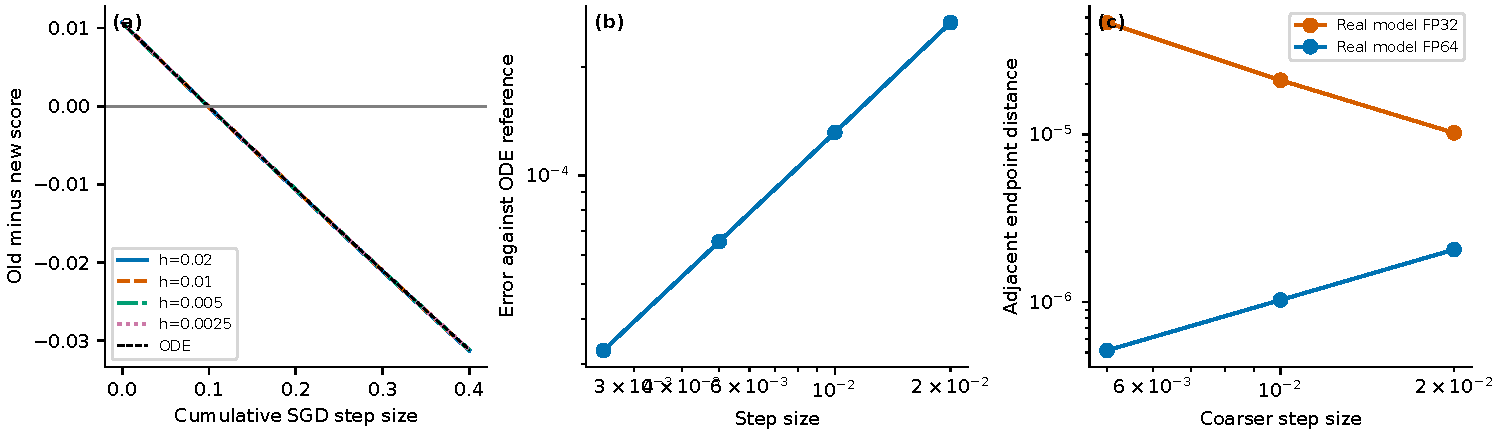
\includegraphics[width=\linewidth]{figures/dynamics_controls.pdf}
\caption{Controls and precision. (a) The fixed quadratic construction
crosses under four FP64 SGD step sizes and the forward ODE reference.
(b) Its endpoint error decreases approximately linearly with step size.
(c) At the selected real-model state, FP32 adjacent-resolution endpoint
differences increase as small updates accumulate; the dtype-preserving
FP64 follow-up restores first-order refinement. The figure includes the earlier FP32 results as well as the FP64 follow-up.}
\label{fig:dynamics-controls}
\end{figure}

\subsection{Ordinary natural-language training: all 18 runs}

The models use the cached revisions, tokenizers and WikiText training
corpus in Appendix~\ref{app:llm-study}. Freeze every backbone. Select 12
attention output projections uniformly across depth using rounded evenly
spaced indices, adapt 64 fixed output rows per projection, and use four
shared bases. Pythia-160M uses all layers; Qwen3-0.6B and SmolLM2-360M use
subsets. Initialize router logits as standard normal and basis entries
with standard deviation $0.01/\sqrt{d_{\rm in}}$, with seeds 0,1,2.
Repeated router initializations across models introduce dependence.

All 18 runs use 256 updates, batch size four and 128 next-token positions
per block. AdamW uses zero decay and default moments; SGD uses no momentum
or decay. Peak basis/router rates are $10^{-3},10^{-2}$, with 16-step
linear warmup and cosine decay to one tenth of the peaks. Clip global
factor-gradient norm at one. Backbone/autocast arithmetic is BF16,
factors FP32. SGD is not separately tuned. The batch generator seed is
$4900000+$adapter seed. No grouping loss, artificial label or constructed
boundary initialization is used.

At initialization and after every update record $A,BB^\top$ in FP64.
Compute global SSE by Equation~\eqref{eq:pairwise-sse}; use exact
capacity-constrained assignment for the coefficient objective. A strict
winner has runner-up gap greater than
$10^{-8}\max(1,|\text{winning objective}|)$. An event requires strictness
of both objectives immediately before and after an agreement-to-disagreement
transition. Also record persistence for five consecutive post-event states.
``Router only'' keeps the weight optimum fixed and changes the coefficient
optimum. ``Response'' refers to the Euclidean objective of
Theorem~\ref{thm:response-partition}, including when assessed along AdamW;
it does not mean AdamW-optimal tying.

\begin{table}[htbp]
\centering\small
\begin{tabular}{llrrrrr}
\toprule
Model & Optimizer & Seed & Coeff. & Router only & Response & Valid NLL before/after \\
\midrule
Pythia-160M & adamw & 0 & -- & -- & 10 & 4.3082/4.3030 \\
Pythia-160M & adamw & 1 & -- & -- & 61 & 4.3090/4.2026 \\
Pythia-160M & adamw & 2 & 6 & -- & 6,52 & 4.3165/4.2819 \\
Pythia-160M & sgd & 0 & -- & -- & -- & 4.3082/4.3291 \\
Pythia-160M & sgd & 1 & -- & -- & -- & 4.3090/4.2969 \\
Pythia-160M & sgd & 2 & -- & -- & -- & 4.3165/4.2986 \\
Qwen3-0.6B & adamw & 0 & -- & -- & 8,80 & 3.5664/2.8878 \\
Qwen3-0.6B & adamw & 1 & -- & -- & 156 & 3.5667/2.9090 \\
Qwen3-0.6B & adamw & 2 & 12 & -- & 12 & 3.5667/2.8973 \\
Qwen3-0.6B & sgd & 0 & -- & -- & -- & 3.5664/3.5517 \\
Qwen3-0.6B & sgd & 1 & -- & -- & -- & 3.5667/3.5510 \\
Qwen3-0.6B & sgd & 2 & -- & -- & -- & 3.5667/3.5474 \\
SmolLM2-360M & adamw & 0 & -- & -- & 5 & 3.0372/2.8057 \\
SmolLM2-360M & adamw & 1 & 71 & 71 & 97 & 3.0359/2.8102 \\
SmolLM2-360M & adamw & 2 & 26 & -- & 26 & 3.0363/2.8040 \\
SmolLM2-360M & sgd & 0 & -- & -- & -- & 3.0372/3.0357 \\
SmolLM2-360M & sgd & 1 & -- & -- & -- & 3.0359/3.0352 \\
SmolLM2-360M & sgd & 2 & -- & -- & -- & 3.0363/3.0369 \\
\bottomrule\end{tabular}
\caption{All 18 exploratory runs. Event columns give every transition step, not independent samples. Validation uses 32 fixed WikiText validation blocks per model, not a full-corpus benchmark. Identical seeds reuse the same initial router across models; architecture, pretraining, and selected layers differ. SGD uses the original schedule without retuning.}
\label{tab:all-dynamics-runs}
\end{table}


All runs complete. The Pythia-160M seed-1 AdamW response event does not
sustain five states; each other AdamW run has a sustained response event.
SGD has no detected event of any declared type. Validation NLL in
Table~\ref{tab:all-dynamics-runs} averages 32 fixed validation blocks,
not the official full-corpus benchmark. Nine AdamW and seven SGD runs
improve this diagnostic; no significance or optimizer-quality claim follows.
Training NLL stored at an update is measured on that minibatch
\emph{before} the update; the geometric record is the after-update state.

For the first occurrence of each event type, save both factor states,
preceding optimizer state, clipped gradients and batch indices. There are
14 records, including one physical update saved under multiple event types.
CPU optimizer replay reproduces all within $2\times10^{-6}$ absolute error.
Independently recomputing 120 initial/final/event-boundary clustering costs
using projector traces rather than pair distances gives the same winners
and maximum cost difference $7.11\times10^{-14}$. These are implementation
checks, not additional training replicates.

\subsection{Selected real-model local Euclidean reproduction}

In SmolLM2 seed-1 AdamW, coefficient and weight partitions initially
disagree, later agree, and diverge again at update 71. The local initial state is its
actual update-70 state, not the random initialization. A fresh GPU pass
on the recorded update-71 batch reproduces loss, gradients and restored
AdamW update exactly in the same environment. The coefficient-gap derivative
under its clipped negative logit gradient is $-1.57367\times10^{-4}$.
This motivates the explicitly \emph{post hoc} follow-up.

Keep the trained state, pretrained weights and original four text blocks.
Fix the batch and optimize the same mean next-token cross entropy, using
equal basis/logit rates, no momentum, clipping or decay, and no autocast or
TF32. Rates $0.02,0.01,0.005,0.0025$ run to time $0.4$. All four FP32
runs cross with the weight partition fixed; a 20-step zero-rate FP32 control
does not move. Adjacent-resolution endpoint distances
$1.0221\times10^{-5},2.1078\times10^{-5},4.6522\times10^{-5}$ instead
increase with refinement, so FP32 does not establish numerical convergence.

We kept the FP32 results and ran two precision follow-ups. First convert the backbone
and factors to FP64 and remove the shared injection's FP32 cast. Source
inspection reveals that RMSNorm still computes in FP32. Its crossings
and approximate first-order refinement are retained as outer-FP64 results.
Second, evaluate the identical RMS formula in the input dtype at all 65
normalization modules, preserving their weights and epsilon. Fixed rotary
position constants may originate from FP32 but do not depend on trained
factors. Cached BF16 pretrained weight values are merely converted to
FP64; no extra pretrained information is introduced.

\begin{table}[t]
\centering\small
\begin{tabular}{rrrrr}
\toprule
Step size & Updates & First crossing & Training time & Adjacent endpoint distance \\
\midrule
0.0200 & 20 & 9 & 0.180 & $2.06\times10^{-6}$ \\
0.0100 & 40 & 17 & 0.170 & $1.03\times10^{-6}$ \\
0.0050 & 80 & 34 & 0.170 & $5.14\times10^{-7}$ \\
0.0025 & 160 & 68 & 0.170 & -- \\
\bottomrule\end{tabular}
\caption{Selected real-model local SGD with FP64 factors, backbone arithmetic and dtype-preserving RMSNorm. Training time is update count times step size. Endpoint distances compare each run to the next finer step size at time $0.4$, not to an exact flow solution. All four runs keep the weight partition fixed.}
\label{tab:local-flow-refinement}
\end{table}


In dtype-preserving FP64, the initial coefficient-gap velocity is
$-1.57929\times10^{-4}$, predicting linearized crossing time $0.16556$.
Observed first crossing times are $0.18,0.17,0.17,0.17$;
Table~\ref{tab:local-flow-refinement} reports empirical refinement.
The weight optimum stays fixed at every recorded state. Minimum router
entry is $0.006781$; minimum singular values of $A,B$ are
$0.856727,2.054078$. Fixed-batch NLL decreases from $3.288429$ to about
$3.286897$. This is local training/arithmetic evidence, not a generalization
gain attributable to a sharing decision.

The experiment connects a state reached during language training to a
local Euclidean crossing under the same language loss. Because the state
was selected, it cannot estimate crossing probability or resolve the
absence of crossings in the nine ordinary-SGD runs. It also leaves
downstream decision quality untested. We use native factors to study
the crossing; the effect of recovery error near the boundary remains open.

\subsection{Artifact and compute boundaries}

The local machine has eight RTX 5090 GPUs with approximately 32\,GiB each.
Ordinary trajectory runs use three GPUs concurrently; recorded per-job
elapsed times sum to 419.12 seconds, including loading/evaluation.
This is not wall-clock makespan or total GPU active time. Precision
follow-ups use separate single GPUs; constructed regression uses CPU.
We do not claim a complete research-compute total.

Protocols, every run, all precision variants and source/input hashes are
retained. Experiments-directory entry points include
\texttt{train\_routing\_crossing.py},
\texttt{train\_llm\_routing\_trajectory.py},
\texttt{replay\_llm\_routing\_backward.py}, and
\texttt{train\_llm\_local\_flow\_fp64\_norm.py}.
\texttt{generate\_dynamics\_paper.py --check} reconstructs tables and
vector figures. Frozen recovery sources/raw results are preserved;
training refuses to overwrite completed results, so rerun in a fresh
output/worktree. The record verifier distinguishes historical manuscript
hashes from the current integrated paper. Artifact checks and AI-assisted
self-review are not external human peer review.
